\secrel{Добавление в схему транзистора}

\begin{framed}
\termdef{Транзистор}{транзистор}\ --- электронный элемент, выполняющий функцию
\termdef{усиления}{усиление}: \emph{управление сильным сигналом под контролем
слабого сигнала}.
\end{framed}

\bigskip
Один из видов\ --- \termdef{Полевой транзистор}{полевой транзистор} 
(\termdef{FET}{FET}, [F]ield [E]ffect [T]ransistor). Управление выполняется
слабым \emph{входным напряжением}, которое управляет \emph{выходным током},
изменяя проводимость (сопротивление) части транзистора в выходной цепи. 

Главная особенность полевого транзистора\ --- во входной цепи, по которой
подается управляющее напряжение, течет почти нулевой \termdef{входной
ток}{входной ток}, т.е. \emph{полевой транзистор имеет бесконечное
\termdef{входное сопротивление}{входное сопротивление}}. Эта особенность важна
при подключении источников слабого сигнала (датчиков), генерирующих слабое
сигнальное напряжение, но не способных выдать сколь нибудь заметный ток\ ---
электро-динамический микрофон, индуктивный звукосниматель электрогитары и т.п.
Сигнал от таких датчиков усиливается \termdef{предварительным
усилителем}{предварительный усилитель} на полевом транзисторе, а затем усиленный
сигнал подается в остальную часть схемы для дальнейшей обработки.

\bigskip
У FET-транзитора три ноги:

\begin{tabular}{l l l}
S & Source & исток \\
G & Gate & затвор \\
D & Drain & сток \\
\end{tabular}
\bigskip

Слабый сигнал не затворе способен управлять б\'{о}льшим током, текущим с истока
на сток. Ток стока тот же самый, который течет через светодиод. Резистор 390\,Ом
ограничивает этот ток на приемлемом для работы светодиода уровне.

\bigskip
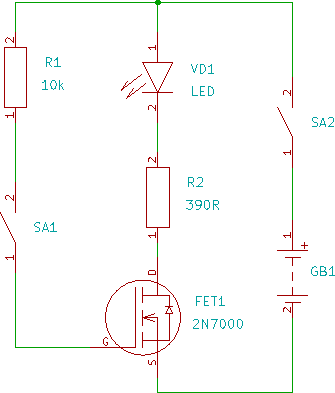
\includegraphics[width=0.45\textwidth]{bcollis/fet/fet.pdf}
\bigskip
